% !TEX root = comparison.tex
%% \section{Introduction} %for journal use above \firstsection{..} instead
%We introduce and discuss a tool for comparing different charts that are renderings of the same data in order to evaluate them for efficiency.
Graphics have a central role in the discovery process as well as in the presentation of results. 
As designer of  charts one of our main goals is to display data so that the information it contains is relayed in the most efficient way. 
In the search for the best display out of the seemingly endless multitude of methods we are guided by experience, knowledge of perceptual strengths and weaknesses, as well as aesthetic preferences. It is hard, if not impossible, to make the final decision on the design in an  objective manner. 
We can make this process less subjective by conducting user studies to evaluate competing designs of the same data, and measure designs for their efficiency by recording how accurately and quickly viewers can extract pieces of information. 
User studies for evaluating different designs has a long standing tradition. For  statistical graphics user studies have their origin in the (convenience) study on evaluating difficulty of a set of different visual tasks by \citet{cleveland:1984}, which has recently been replicated with similar results based on a large MTurk study by \citet{heer:2010}.

Usually, we need simulation studies to be able to completely control for the signal strength in the data. 
For charts, this is not a very realistic scenario. The need for displaying information particularly efficiently or accurately usually arises from  a particular problem while analyzing a data set, from which we want to learn new insight. Often, it is difficult to simulate data in such a way that it realistically represents the particular problem, which in turn makes it dubious whether the results from a simulation study are actually applicable to the problem at hand, reminding us painfully of George Box's famous quote on models: ``essentially, all models are wrong, but some are useful.'' \citep[page=424]{box}  

Lineup tests  \citep{buja:2009} allow us to directly use the data at hand to evaluate different competing designs by using permutations tests \cite{good:2011} of the original dataset. We can therefore get valid quantitative measures for comparing different designs without having to set up a simulation.

When we are presenting a chart we  want to convince our audience of the presence of a particular feature or relationship in the data. 
In order to enable us to draw a conclusion about presence or absence of a feature in the data, we have, however, to assess what features show up based purely on marginal distributions rather than joint distributions.

\begin{figure}[htbp] %  figure placement: here, top, bottom, or page
   \centering
   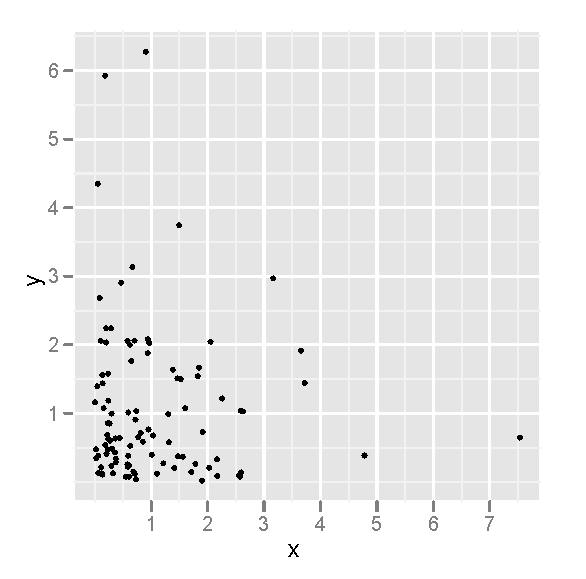
\includegraphics[height=0.32\linewidth]{rexp.pdf} 
   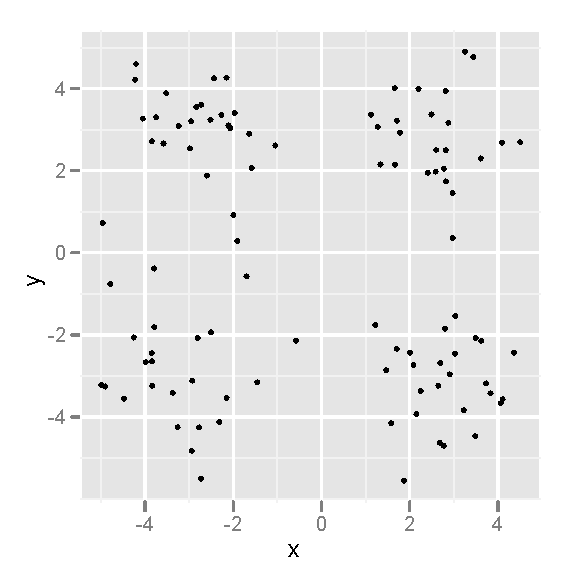
\includegraphics[height=0.32\linewidth]{rnorm.pdf} 
   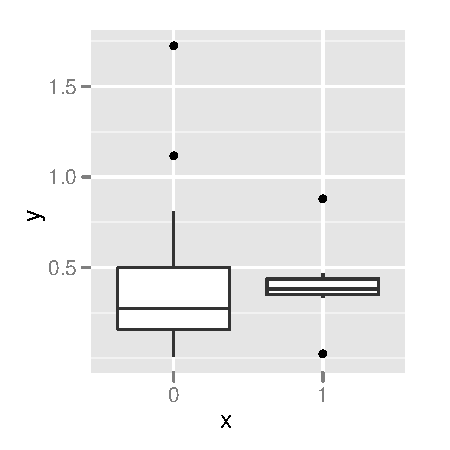
\includegraphics[height=0.32\linewidth]{two-exp.pdf} 
   \caption{Examples of charts with distinctive features but independent variables. From left to right: scatterplot of $X$ and $Y$ with independent $X, Y \sim Exp_{\lambda=1}$; scatterplot of two variables with mixed normal distribution $N(3,1)$ and $N(-3,1)$; boxplot of $X$ and $Y$ with $X \sim B_{n=100, p=0.1}$ and $Y \sim Exp_{\lambda=1}$. }
   \label{random}
\end{figure}

Features in the marginal distributions, such as multi-modality, skewness  or outliers, might interfere with our intuition of what `randomness' might mean in a particular situation and lead us to wrong conclusions. All of the plots in figure \ref{random} show distinctive features. None, of these, however, is a feature of the joint distribution, i.e. all of the variables involved are independent of each other. The scatterplot on the left of figure \ref{random} shows data sampled from an exponential distribution with rate parameter $\lambda=1$. The data in the middle comes from mixing two normal distributions with different means: half of the points has mean $\mu_1 = -3$, the other half has mean $\mu_2=3$, which results in the distinctive four groups.
The two boxplots on the right appear to show a median shift between the two groups. This, however is a result of both the group size (only 7\% of the points is in the second group) and a skew distribution in vertical direction, with $y \sim Exp_{\lambda=1}$. 


Lineup plots have been shown as an effective tool \cite{wickham:2010} for enabling us to quantitively assess the strength of the relationship between $X$ and $Y$.
In a lineup plot the plot of the actual data is -- as in a police line-up -- inserted among decoy plots. The decoy or {\it null} plots are generated in a way that is consistent with the null hypothesis, i.e. these are plots in which we can assume that any relationship visible is there purely by chance. This gives us a reference framework against which to compare the data plot and, if we are still able to identify the data plot from the lineup because of a distinguishing feature, we have formal evidence that the feature in the data is, in fact, not just coincidental. 

The strength of this evidence is determined by both the number of independent evaluations as well as the size of the lineup. 
Assume a lineup of size $m$ is evaluated by $n$ independent observers, out of which $x$ identify the data plot correctly, which we can use as an estimate for the probability to correctly identify the data plot:
this leads us to an estimate for the probability of correctly identifying the plot of $x/n$, with 95\% confidence intervals  for $x/n$ given as $x/n \pm 1.96 \cdot \sqrt{x/n \cdot (1-x/n)}$ limited to the interval [0,1]. Note, that the resulting interval is often too large to be useful.

We can think of a lineup as $m-1$ head-to-head comparisons of the dataplot and $m-1$ nullplots, which the dataplot all has to `win', in order to be picked as the plot with the most distinct features. Assuming that observers identify the plot with the strongest signal, the probability that data plot is picked follows a Beta distribution for the maximum:
this allows us to introduce the {\it signal strength} \cite{majumder:2011} of a lineup as:
\[
\text{signal strength} =  \left( \frac{x}{n}\right)^{1/(m-1)}.
\]
Signal strength is limited to a range of values between 0 and 1. Higher values indicate stronger signal.
 In the case of a parametric situation (i.e. the feature shown in the chart can be described in parametric form as a real-valued vector $\theta$ in the data), it can be shown \cite{majumder:2011} that the signal strength is strongly correlated to the $p$-value of the corresponding statistical test for $\theta$.
 
\section{Comparison of Designs}
We are going to make use of the signal strength gained from multiple viewings of a lineup in order to evaluate competing designs as follows:
\begin{enumerate}
\item{{\bf Create Lineup Data:} create data for a lineup of size $m$ by  creating  $m-1$ permutations of $y$ or, in the case of a simulation study, drawing $m-1$ samples of size $n$ (the number of rows in the data) from the null distribution. Add the original data to the lineup data randomly between 1 and $m$. }
\item{{\bf Create lineups from competing designs:} using the same data, render lineups of all competing designs. }
\item{{\bf Evaluate Lineups:} by presenting the lineups to independent observers. Assess both signal strength and time needed by individuals to come to a decision. Note that each observer should only be exposed to each lineup data once.}
\item{{\bf Evaluate Competing Designs:} differences in signal strength or time to decision are due to differences in the design. In the case that individuals were shown multiple lineups (as part of a bigger study), it is possible to correct outcome measurements for an individual's visual ability. }
\end{enumerate}

XXXX should we include nullabor code?

The power of a statistical test is defined as the probability to reject the null hypothesis. Translated to the visual tests, power is the probability to identify the data plot from the lineup. 
Comparing power of competing designs therefore involves comparing percentages of correct responses $p_1$ and $p_2$. An $\alpha\cdot$100\% confidence interval for this comparison is given as 
\[
p_1 - p_2 \pm t_{1-\alpha/2, n-1} \sqrt{p_1(1-p_1)/n_1 + p_2(1-p_2)/n_2},
\]
where $n$ is the Welch-Satterthwaite \cite{welch:1947} estimate of the degrees of freedom. Note that we use $p_i = (x_i+1)/(n_i+1)$ and $n_i+2$ for a better coverage of the confidence interval \cite{agresti:1998}.

While this allows a direct comparison of the designs, we cannot adjust for the individuals' perceptual abilities.
In the case that we have multiple responses from each person (i.e. data is collected on several {\it different} lineup tasks), we can estimate for their perceptual ability and correct power differences between competing designs accordingly, e.g. by modeling power using  a subject-specific random intercept in a generalized linear model.




%We also know that humans learn about new information through a visual search pattern that emphasizes new information (Wolfe, 2002; Rensick, et al., 1997). Of course, the type of visualization should take the natural human inclinations into account as well. For instance, a good visualization will account for both the �gestalt? like perceptual tendencies as well as the detail-orientated nature of cognition (Kosslyn, Thompson and Ganis, 2002; Pylshyn,2003)



